\documentclass{beamer}
 
\usepackage[utf8]{inputenc}

\usepackage{polyglossia}
\setdefaultlanguage{english}
\setotherlanguage{russian}

\usepackage{graphicx}
\setlength\fboxsep{3pt}
\setlength\fboxrule{1pt}

\usepackage{pythonhighlight}
\usepackage{listings}
\usepackage{lstautogobble}
\usepackage{color}
\usepackage{zi4}
\lstset{
    autogobble,
    columns=fullflexible,
    showtabs=false,
    breaklines=true,
    showstringspaces=false,
    breakatwhitespace=true,
    escapeinside={(*@}{@*)},
    tabsize=4,
}

\usepackage[autostyle]{csquotes}
\usepackage[backend=biber,style=authoryear]{biblatex}
\addbibresource{mybiblio.bib}
 
\title{Python Library for Linguistic Typology}
\author{Michael Voronov}
\institute{Higher School of Economics}
\date{18.06.2019}
 
\begin{document}
 
\frame{\titlepage}
 
\begin{frame}
\frametitle{Introduction}
Problem:
\begin{itemize}
 \item No Python tools for online linguistic databases queries.
 \item No Python tools for linguistic interactive mapping.
\end{itemize}
What exists?
\begin{itemize}
 \item R package \textbf{lingtypology} that does both \parencite{GeorgeMoroz2018}.
\end{itemize}
Why Python?
\begin{itemize}
 \item De-facto standard language among linguists.
 \item A lot of scientific libraries (Pandas, SciPy etc.)
 \item Unicode out of the box.
 \item Relatively high speed.
 \item Versatile language.
\end{itemize}
\end{frame}
 
\begin{frame}
\frametitle{Used Tools}
\begin{itemize}
 \item Python \parencite{python}
 \item Pandas \parencite{pandas}
 \item Folium \parencite{folium}
 \item Matplotlib \parencite{matplotlib}
 \item PyGlottolog \parencite{Robert2Forkel2019}
 \item OpenElevationAPI \parencite{OpenElevation}
 \item SciPy \parencite{scipy}
\end{itemize}
\end{frame}


\begin{frame}
\frametitle{Project Description}
Remote Repository:
\begin{itemize}
 \item https://github.com/OneAdder/lingtypology
\end{itemize}
Documentation:
\begin{itemize}
 \item https://oneadder.github.io/lingtypology/
\end{itemize}
Modules:
\begin{itemize}
 \item \texttt{lingtypology.maps}
 \item \texttt{lingtypology.datasets}
 \item \texttt{lingtypology.glottolog}
\end{itemize}
\end{frame}

\begin{frame}[fragile]
\frametitle{Maps}
\begin{python}
languages = ('Romanian', 'Afrikaans', 'Tlingit', 'Japanese')
m = lingtypology.LingMap(languages)
m.create_map()
\end{python}
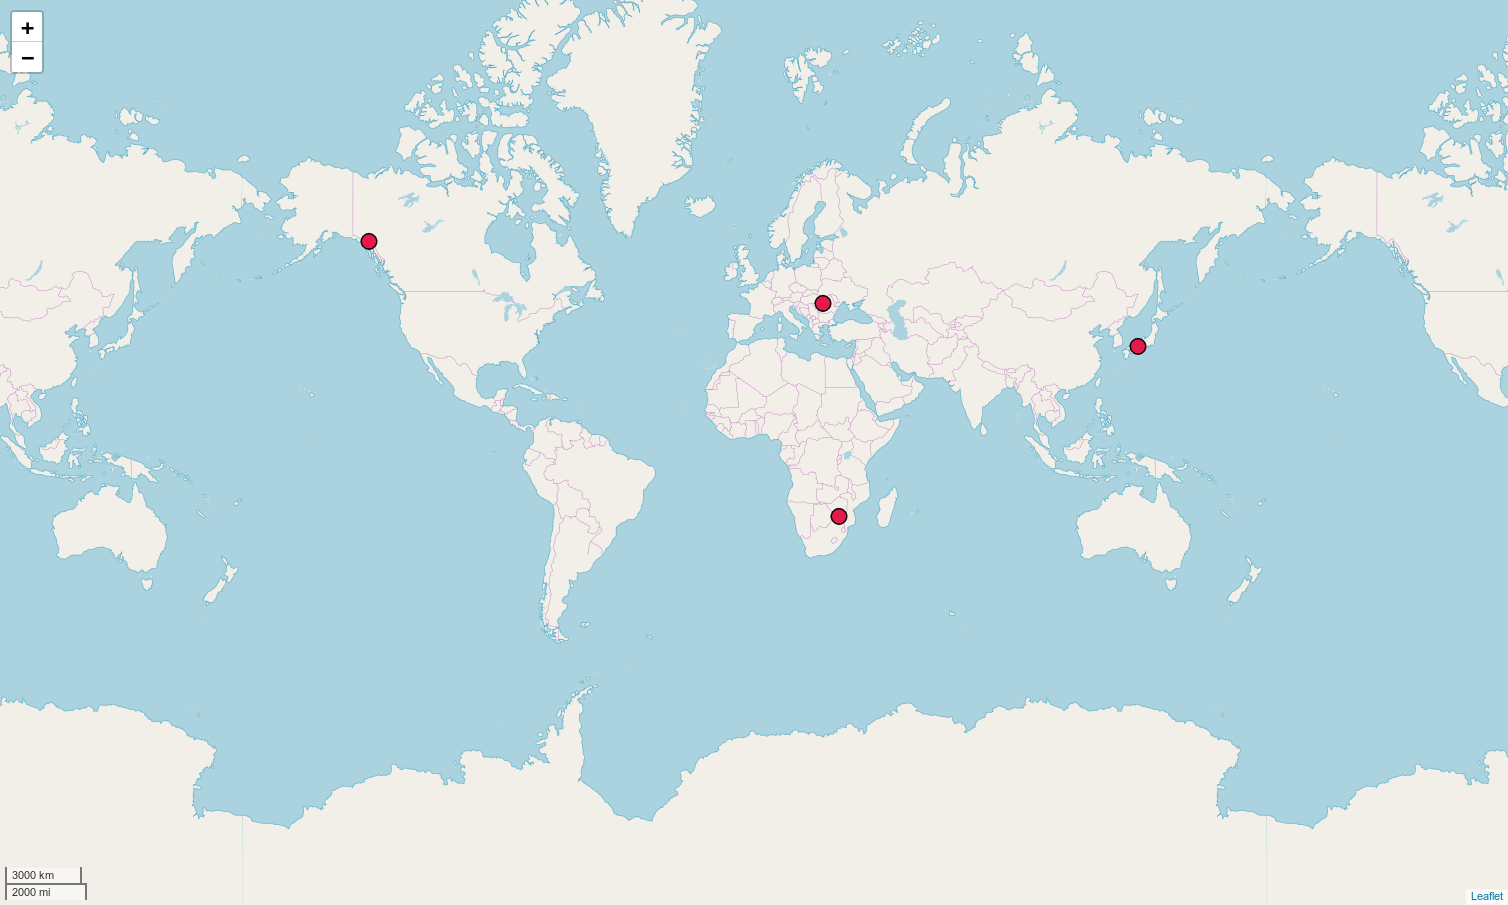
\includegraphics[width=\textwidth]{images/SimpleMap.png}
\end{frame}

\begin{frame}[fragile]
\frametitle{Maps}
\begin{python}
languages = [
    "Adyghe", "Kabardian", "Polish",
    "Russian", "Bulgarian"
]
features = [
    "Agglutinative", "Agglutinative", "Inflected",
    "Inflected", "Analytic"
]
m = lingtypology.LingMap(languages)
m.add_features(features)
m.create_map()
\end{python}
\end{frame}

\begin{frame}
\frametitle{Maps}
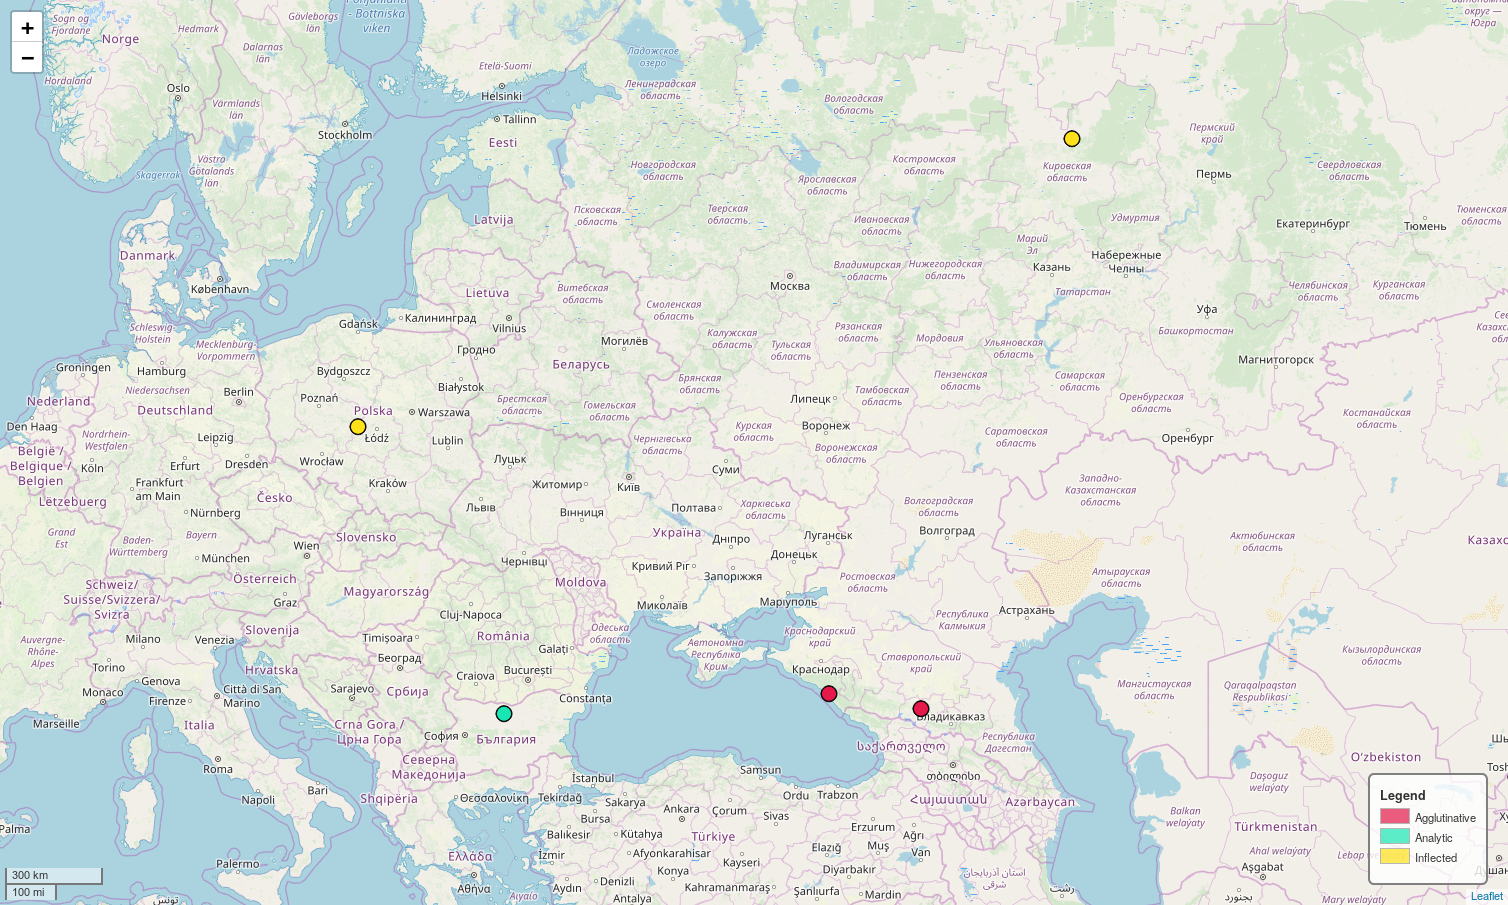
\includegraphics[width=\textwidth]{images/FeaturesMap.png}
\end{frame}


\end{document}
